\section{Discussion} 
\subsection{Evaluation Results}  \

There are two scenarios to construct user need. For the scholarly graph, including a citation (vertex-based query) model and a keyword (text-based query) model. In the citation model, for each user, we first extract all the papers he/she cited before, then use their centroid embedding as user need vector  $\vec{I}$. In the keyword model, for each user (author), I first extract all keywords he/she used in all previous papers to form a text query. Then I retrieve the top 100 relevant papers given the query based on probability language model with Dirichlet smoothing. Finally, I average those retrieved papers' vectors as the user need vector $\vec{I}$.

\begin{table}[h]
	% 	\scriptsize
%	\small
	 \centering
	%\vspace{-3em}
	
%	\renewcommand{\tabcolsep}{3.0pt} 
%	\renewcommand\arraystretch{0.0}
	\begin{tabular}{|c|c|c|c|c|c|c|} 
		\hline
		\multirow{2}{*}{\textbf{Model}} & \multicolumn{3}{c|}{\textbf{Scholarly Graph}} 	&\multicolumn{3}{c|}{\textbf{Music Graph}}\\
		\cline{2-7}%\cmidrule(lr){2-7}
		& F1 & Rand	& Jaccard	& F1 & Rand	& Jaccard\\  \hline
		Spinglass&0.4294 & 0.4149 &0.3593 & 0.4282 & 0.5317& 0.2823 \\ 
		FG& 0.4290 & 0.3852& 0.3735 &0.4645&0.4100& 0.3070 \\ 
		Louvain&0.4417 & 0.4546& 0.3627&0.1832 &0.4201 & 0.1174 \\ 
		Walktrap& 0.4304 & 0.3777 & 0.3777&0.3999 & 0.3507& 0.3490 \\
		Infomap&0.4436 & 0.4165& 0.3606& 0.2147 & \textbf{0.6074} &0.1344\\ 
		Bigclam& 0.2314  & 0.2572 & 0.1348 & 0.1499  & 0.2078  & 0.1227 \\
		DeepWalk&0.3904 & 0.3237 & 0.3234&0.3535& 0.3253& 0.3001 \\ 
		Node2vec & 0.4001 & 0.3472 & 0.3433&0.4122 & 0.4101& 0.3087 \\  \hline
		gPCD-Citation&$\textbf{0.5351}^{*}$ & $\textbf{0.4551}^{*}$& $\textbf{0.4086}^{*}$ &-	&-	& -\\
		gPCD-Keyword&0.5069 & 0.4114& 0.3708 &-	&-	& - \\
		gPCD-Listening&-	&-	& - &$\textbf{0.5188}^{*} $& 0.5865& $\textbf{0.3550}^{*} $\\ 
	\hline
	\end{tabular}
	\begin{tablenotes}
		\item[] \begin{footnotesize}
			Note: ``*'' means the p-value through a pairwise t-test is smaller than 0.001.
		\end{footnotesize}
	\end{tablenotes}
	\caption{Personalized Community Evaluation on gPCD and Baselines. }
	\label{tab:community}
\end{table}


For the music task, text information is not available. The centroid embedding of the songs listened to by a target user are taken as user need.

\textbf{Community Accuracy}: I compare the average performance of my model on all testing users with baselines. Table \ref{tab:community} shows the detailed metrics. When running on the Scholarly graph, both Citation model and Keyword model can achieve around 10\% increase on F1-score compared with all baselines. Citation model also performs the best in Rand Index and Jaccard Index. For Music graph, my Listening model also has a significant improvement on F1-score and Jaccard Index. Although it has similar performance on Rand Index compared with Infomap, I believe my model in fact works much better due to the Infomap's poor performance on the rest two metrics. Moreover, I apply pairwise t-tests for all metrics on all testing users. All metrics' p-values in Citation model and the p-values of F1-score and Jaccard Index in Listening model are all smaller than 0.001, which means the improvements of my model performance are significant compared with baselines.


\textbf{Running Time Comparison}: Table \ref{tab:complexity} shows both the theoretical time complexity and real running time. To represent baseline algorithms' time complexity, ``$V$" refers to the vertex set and ``$E$" refers to the edge set in the graph $G(V,E)$. For some models (FG, Walktrap, and Infomap.), their specific time complexities are officially mentioned in the original papers. The time complexity of Louvain and Bigclam are roughly estimated in the original papers as well but those papers don't mention specific numbers. For Spinglass, DeepWalk and Node2vec, I can't find the exact time complexity in existing studies. Hence in this paper, I arbitrarily assign labels based on the their real running speed. Considering the running time, all the baseline algorithms run relatively fast except for the Spinglass algorithm. However, compared with all other models, the distributed gPCD always performs the fastest. Its real running time of is less than one-tenth of the fastest baseline's running time. 

\begin{table}[h]
	% 	\scriptsize
%	\small
	\centering
	%\vspace{-3em}
%	\renewcommand{\tabcolsep}{2pt} 
%	\renewcommand\arraystretch{0.0}
	\begin{tabular}{|c|c|c|c|} 
		\hline
		\textbf{Model}& \textbf{Time Complexity} & \textbf{Scholarly Graph} (s)	& \textbf{Music Graph} (s) \\ \hline
		Spinglass& very slow &12548.68	& 10372.17 \\ 
		FG& $O(|V|log^2|V|)$&280.60	& 272.34 \\ 
		Louvain& linear&80.01	&63.02 \\ 
		Walktrap&$O(|V|^2log|V|)$& 638.44	& 503.24 \\
		Infomap&$O(|V|(|V|+|E|))$ &501.79	&425.63 \\ 
		Bigclam&linear &57.01 	& 112.43 \\ 
		DeepWalk& fast&720.56	& 688.32 \\ 
		Node2vec& slow&	3508.44&3100.12 \\ 
		gPCD&$O(\frac{2^dKP}{M})$ &\textbf{5.25} &\textbf{6.50} \\ 
		\hline
	\end{tabular}
	\caption{Running time analysis on gPCD and all baselines in seconds (s).}
	\label{tab:complexity}
%	\vspace{-3em}
\end{table}

\subsection{Parameter Analysis}  
\begin{figure}
	\subfloat[Depth $d$ in Citation model]{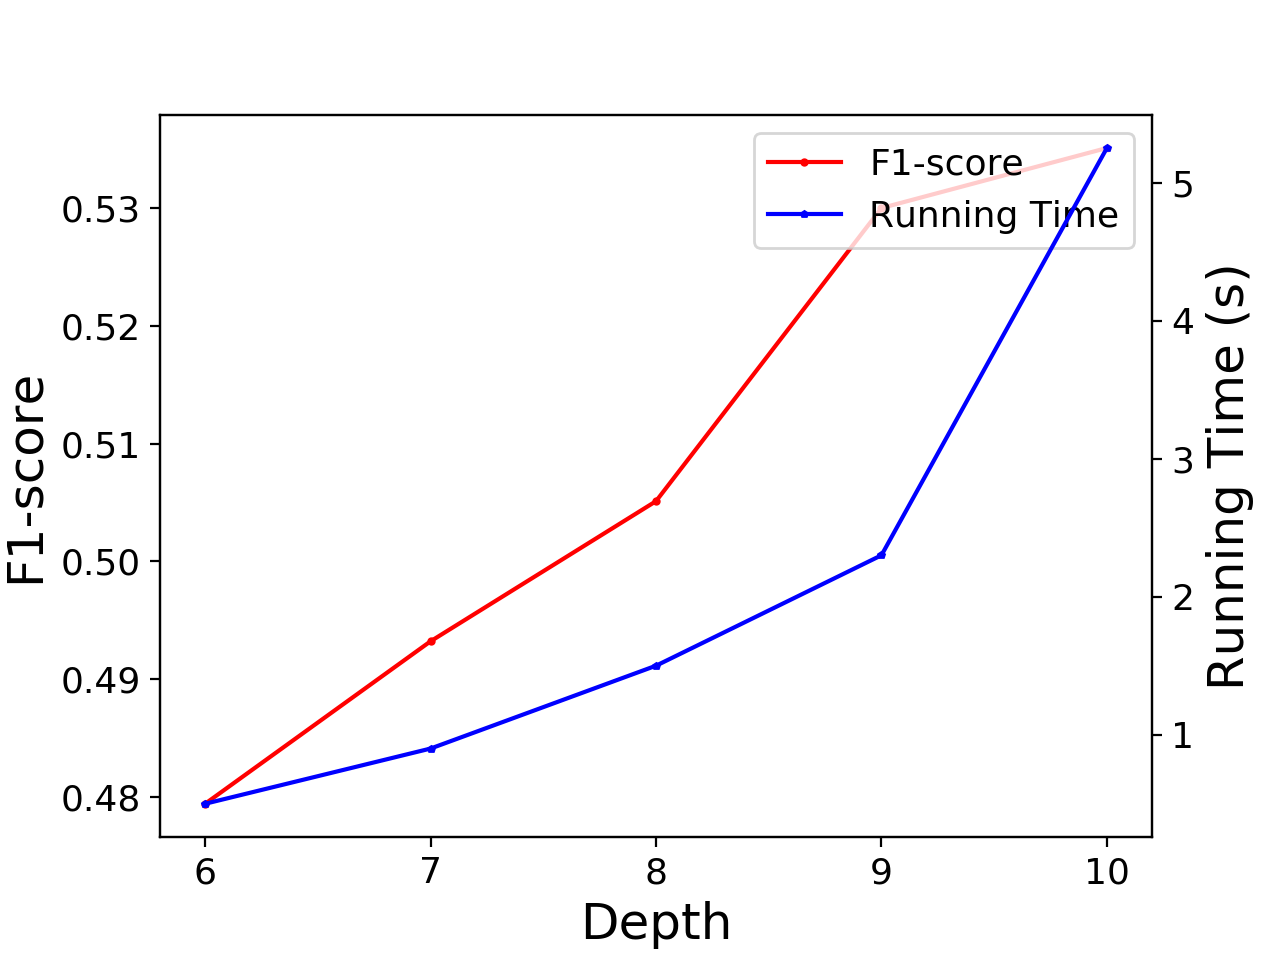
\includegraphics[width = 0.33\columnwidth]{img/chapter3/citation.png}}
	\subfloat[Depth $d$  in Keyword model]{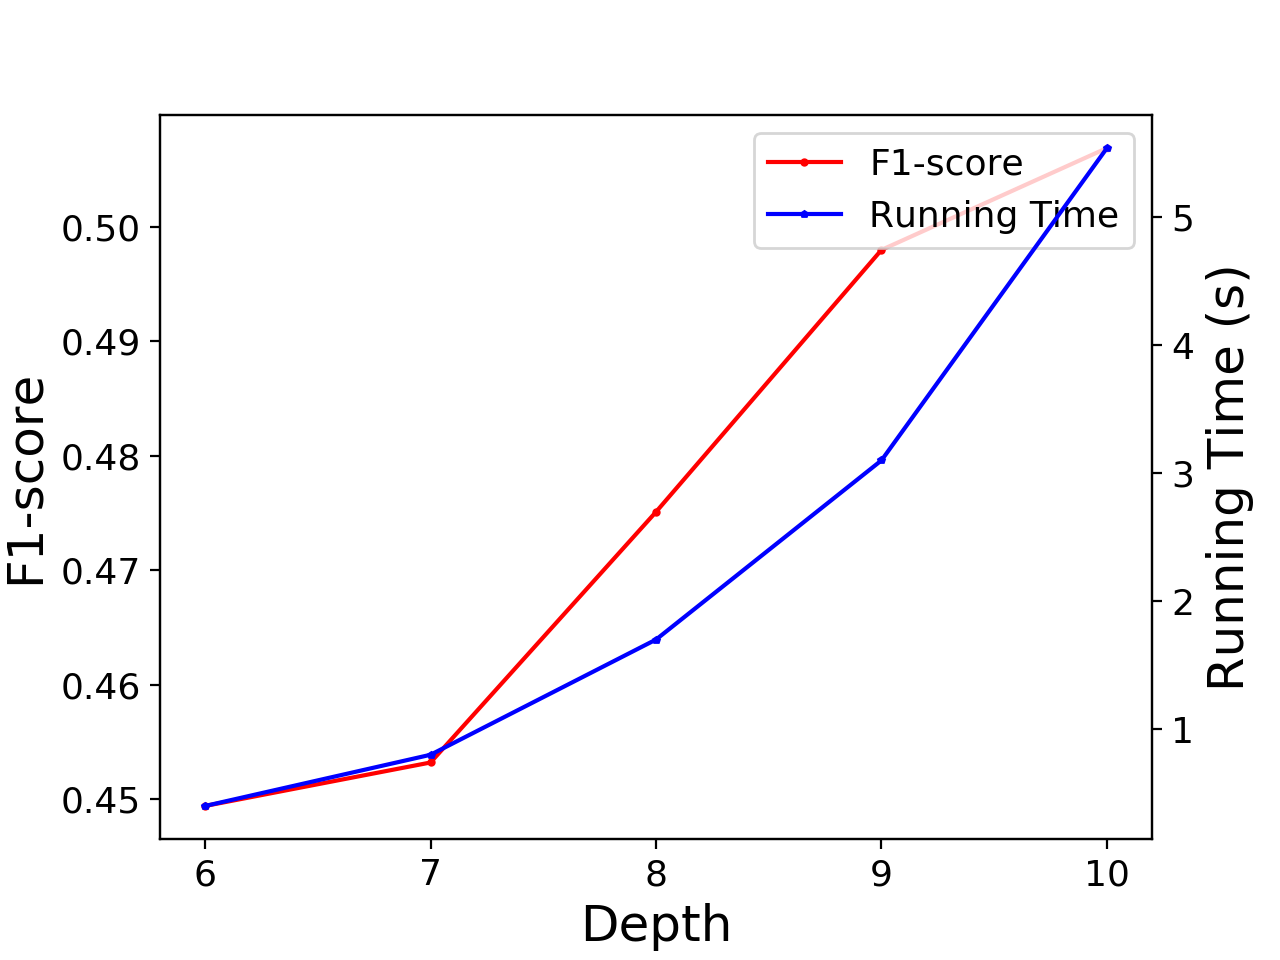
\includegraphics[width = 0.33\columnwidth]{img/chapter3/keyword.png}}
	\subfloat[Depth $d$  in Listening model]{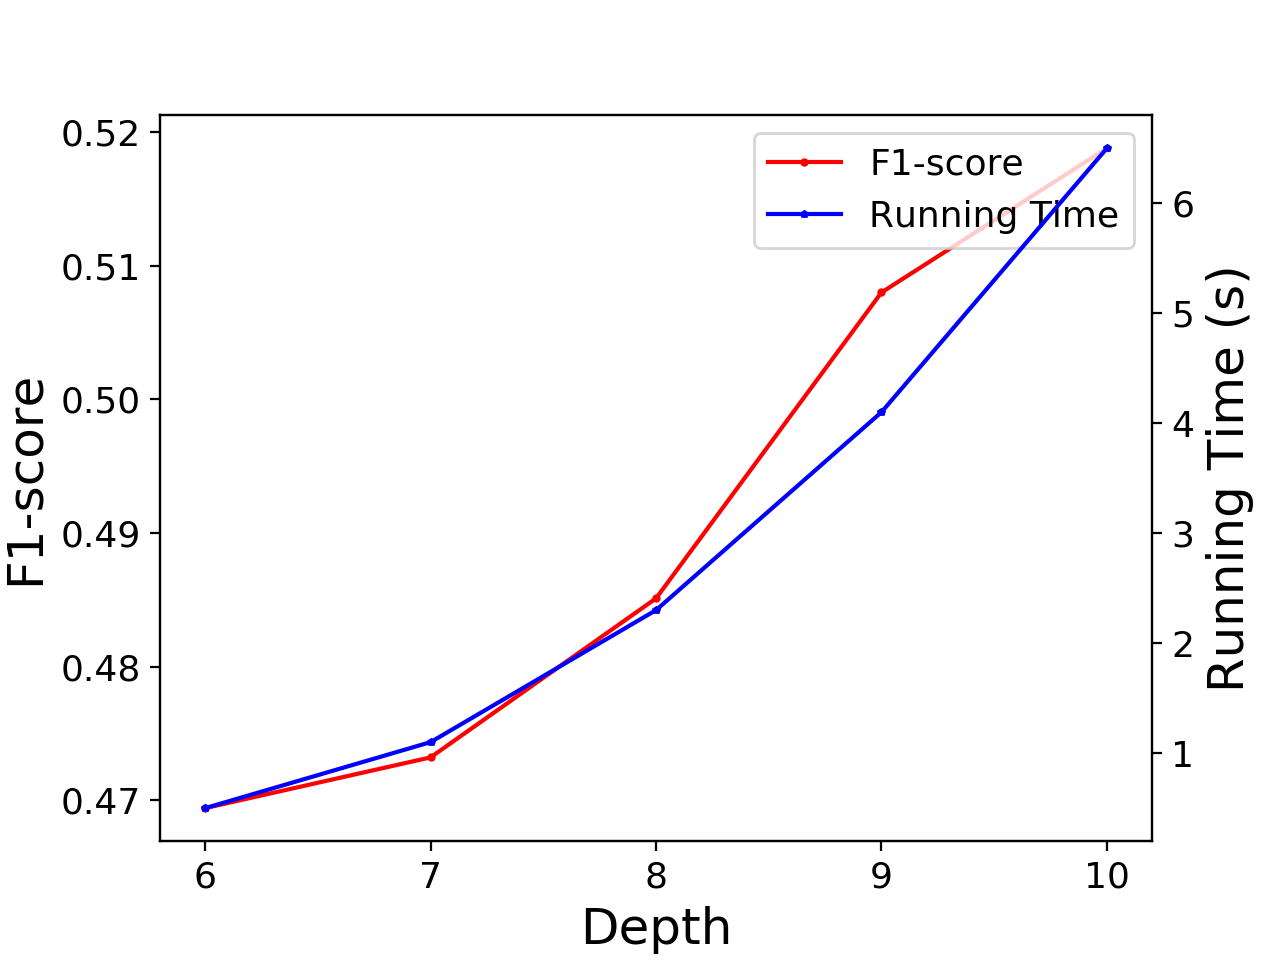
\includegraphics[width = 0.33\columnwidth]{img/chapter3/colisten.png}}  \\
	\subfloat[Iteration $T$ in all models]{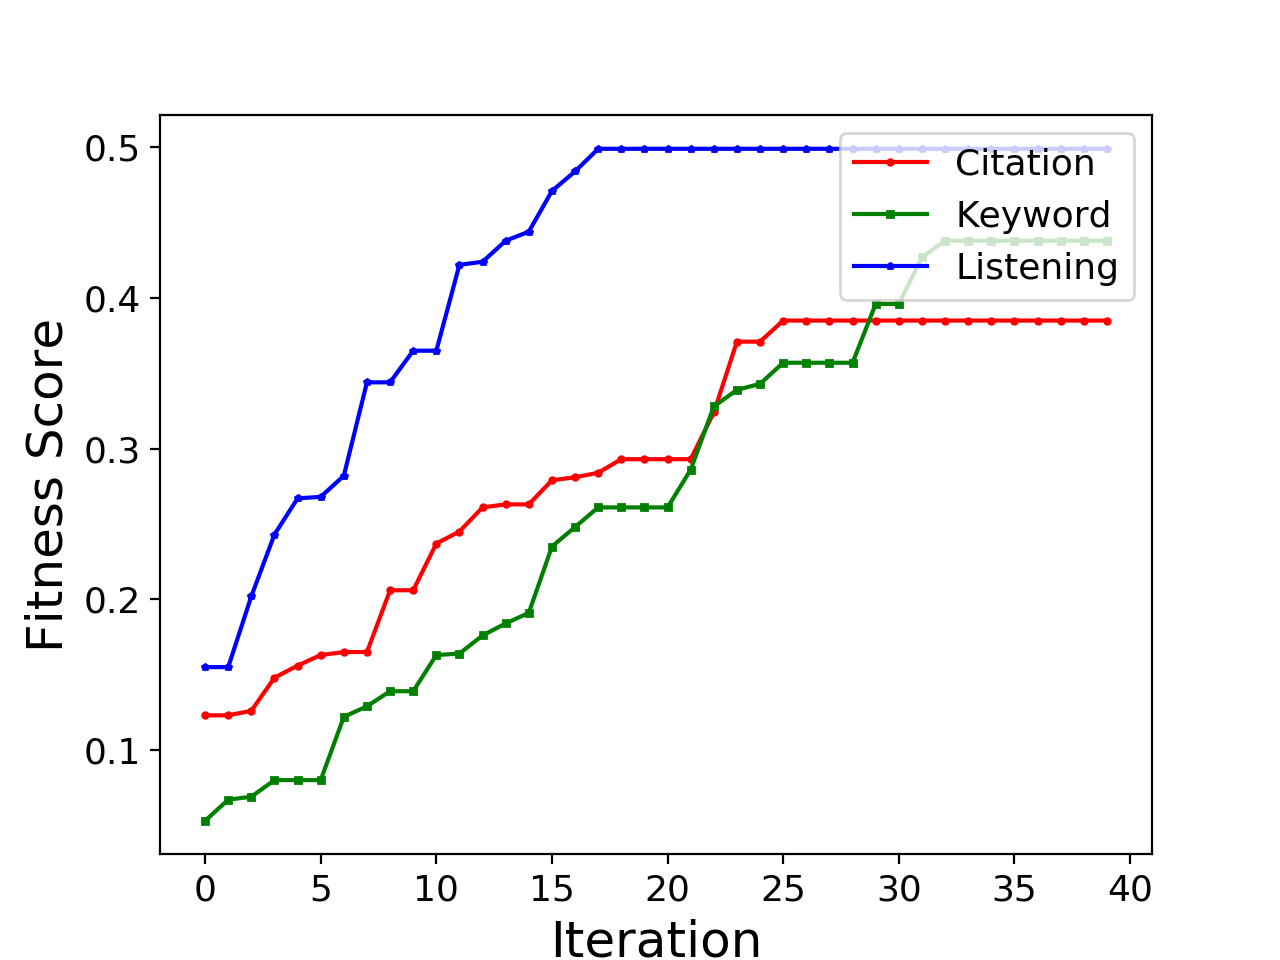
\includegraphics[width = 0.33\columnwidth]{img/chapter3/iteration.png}} 
	\subfloat[User searching preference $\lambda$ in all models]{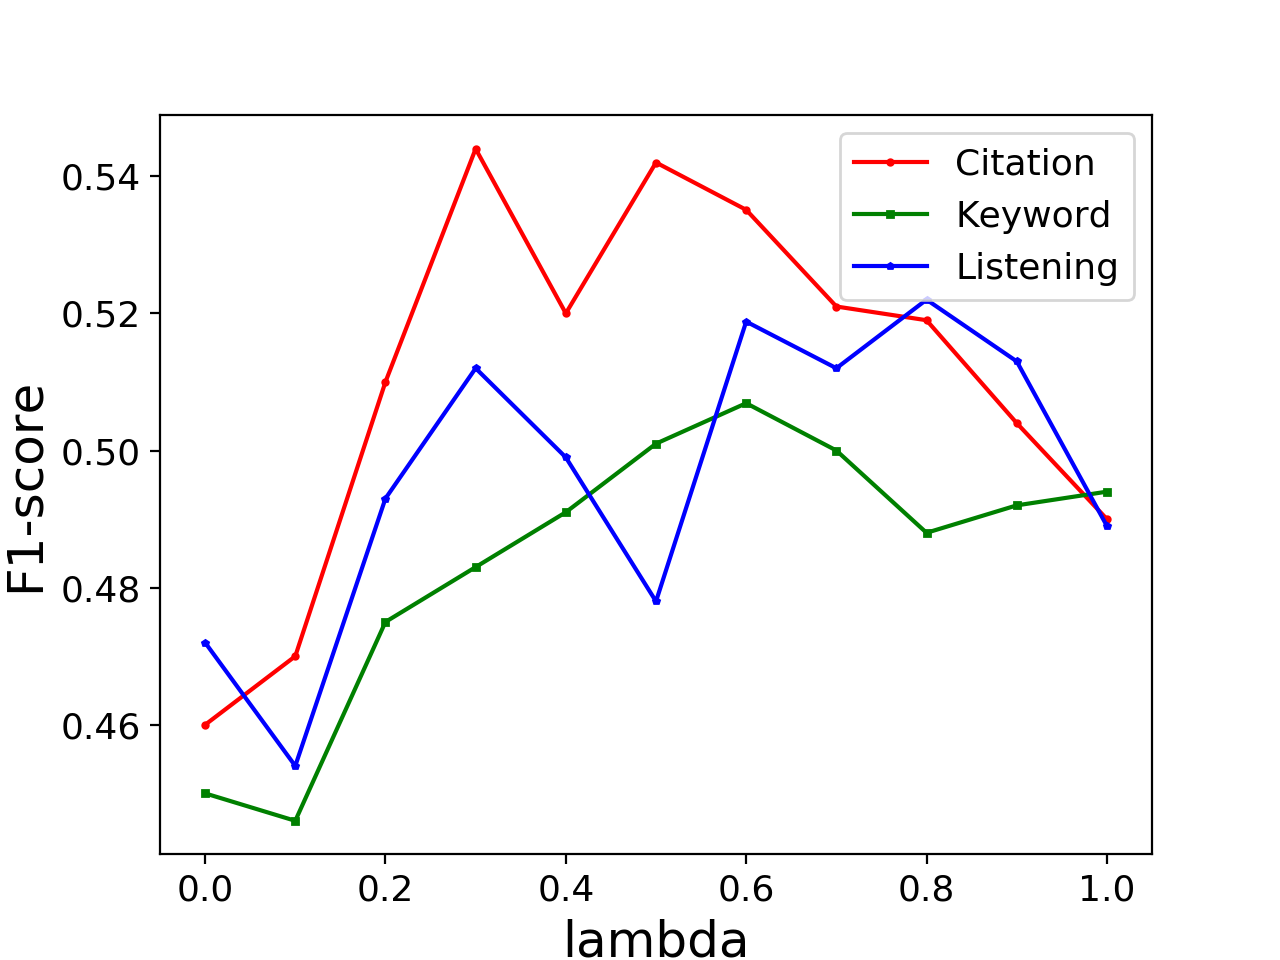
\includegraphics[width = 0.33\columnwidth]{img/chapter3/lambda.png}} 
	%	\vspace{-1em}
	\caption{Parameter effects on model performance}
	\label{fig:tuning}
	%	\vspace{-1em}
\end{figure}
I show how three parameters can affect my gPCD model performance in this section. They are the depth of the binary community tree $d$, genetic iteration number $T$ and user searching preference $\lambda$. Figure \ref{fig:tuning} show the overall impacts of all tuned parameters.



\textbf{Depth on the Tree}: Figure \ref{fig:tuning}(a) to  Figure \ref{fig:tuning}(c) show how the depth of the binary community tree affects the model performance in accuracy and efficiency. From the figures, larger depth leads to a better personalized community detection result, while causes an exponential running time increase at the same time. Based on empirical studies, the upper bound of the depth is set to be 10 in this paper. While the depth selection may varies based on different graph sizes.

\textbf{Convergence Analysis}: I observe the best chromosome updates in 40 iterations. From Figure \ref{fig:tuning}(d),   I can see the fitness score start to be stable after the 30 iterations, which means the best chromosome is no longer changed after around 30 iterations. Thus, I set $T = 30$ as the default iteration number in my approach.

\textbf{Searching Preference}: In Figure \ref{fig:tuning}(e), $\lambda$ reflects the user searching preference whether he/she wants to explore new information or avoid redundant information. By selecting $\lambda$ from 0 to 1, I find  the F1-score are not very stable or have a clear correlation with $\lambda$. Based on the empirical experiments, I achieve the best performance on three models when $\lambda = 0.6$.
